\chapter{From live set to laptop ensemble}

\section{Framework and historical context}\label{framework-and-historical-context}

The history of live sets closely follows technological evolution over the past few decades.

The same instruments, however, are used differently in different musical fields. 

As has always been over the centuries we can consider two distinct aesthetic fields:

\begin{itemize}
\tightlist
\item experimental music.
\item mainstream (popular) music.
\end{itemize}

Sometimes they intersect and contaminate each other but more often continue along their own aesthetic lines.

\subsection{Experimental fields}\label{experimantal-fields}

One of the first works for live electronic performers without acoustic instruments can be considered \href{http://www.musicaecodice.it/gitmedia/emc/6_lvset/suoni/cartridge.mp3}{Cartridge music} (1960) by J.Cage.

\begin{center}
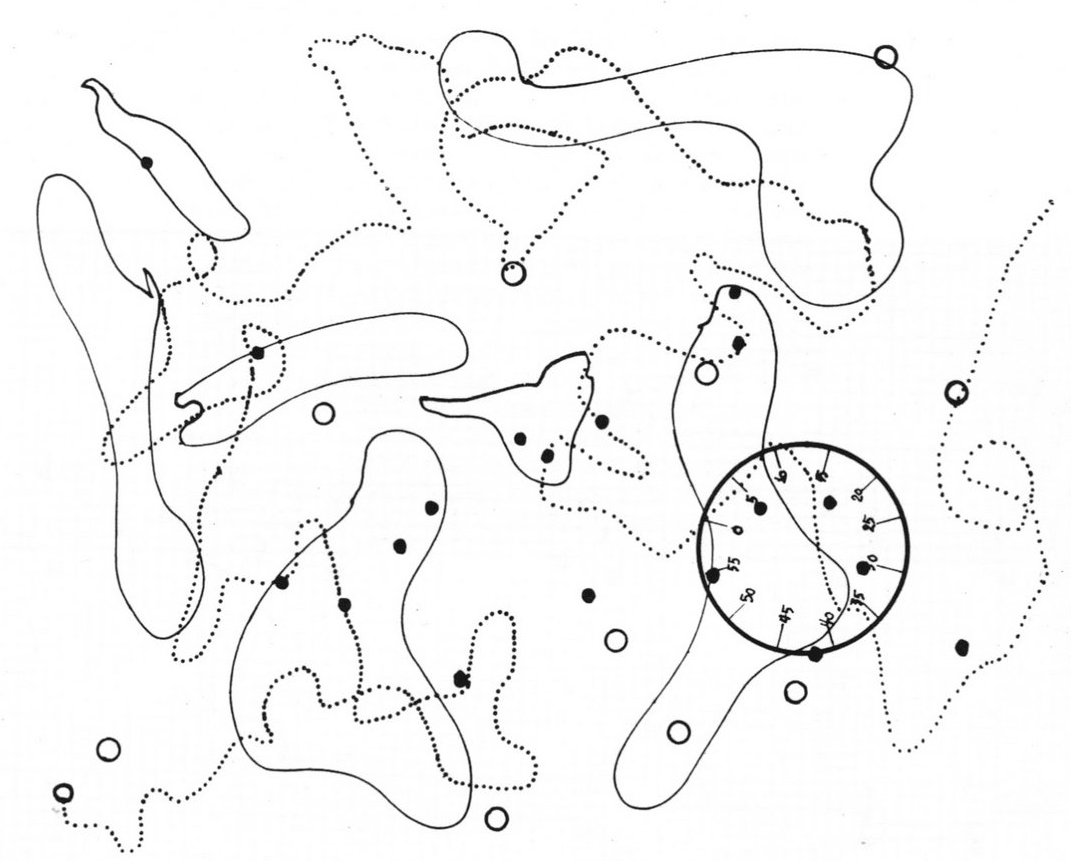
\includegraphics[scale=0.3]{../img/cartridge.png}
\end{center}

It is a composition for small amplified sounds and an indeterminate number of turntables and speakers.

Performers insert some small objects such as matches, wires, feathers and other things inside the metal case of the microphones (cartridge) contained in the old gramophones.



\subsection{Historical framework}\label{historical-framework}

\section{Interaction types}\label{interaction-types}

There are three main ways to control sound parameters:

\begin{itemize}
\tightlist
\item trigger. 
\item switch.
\item continuos.
\end{itemize}

These ways are representative of different types of possible interaction.

Iterations with any type of device and with any communication protocol can be reduced to these modes.

\subsection{Trigger}\label{trigger}

It can be described as pressing a button to ring the doorbell.

One action \(\rightarrow\) do it!

In sound synthesis it is closely connected with envelopes without sustain.

Let's think of it as the action of plucking a string.

Look at it.

\begin{lstlisting}[frame=single] 
s.boot;
s.scope;
s.plotTree;

{Impulse.kr(2,0.5)}.plot(0.5); 
\end{lstlisting}

Audio example.

\begin{lstlisting}[frame=single] 
SynthDef.new(\trig,{var sig, env;
                        env = Env.perc;
                        env = EnvGen.kr(env,doneAction:2);
                        sig = Pulse.ar([600,602],env);
                        sig = sig * env * 0.5;
                    Out.ar(0,sig)
            }).add;
            
Synth.new(\trig);
\end{lstlisting}

\subsection{Switch}\label{switch}

It can be described as pressing a button to switch on/off a light.

Two actions \(\rightarrow\) two staes (on and off).

In sound synthesis it is closely connected with envelopes with sustain.

Let's think of it as the action of press and release an Organ key.

Look at it.

\begin{lstlisting}[frame=single] 
{Trig1.kr(Impulse.kr(2,0.7),0.2)}.plot(0.5); 
\end{lstlisting}

Audio example.

\begin{lstlisting}[frame=single] 
SynthDef.new(\switch, {arg gate=0;
                       var sig, env;
                           env = Env.adsr;
                           env = EnvGen.kr(env,gate,doneAction:2);
                           sig = VarSaw.ar([1300,1310],env);
                           sig = sig * env * 0.5;
                       Out.ar(0,sig)
            }).add;
 
a = Synth.new(\switch, [\gate,1]);
a.set(\gate,0);           
\end{lstlisting}

\subsection{Continuos}\label{continuos}

It can be described as gradually increasing or decreasing the intensity of a light through a knob.

One actions \(\rightarrow\) two staes (movement and stop).

In sound synthesis it is closely connected with interpolation and ramps.

Let's think of it as the action of crescendo, diminuendo or glissato.

Look at it.

\begin{lstlisting}[frame=single] 
{LFNoise2.kr(5)}.plot(0.5); 
\end{lstlisting}

Audio example.

\begin{lstlisting}[frame=single] 
SynthDef.new(\cont,{arg gate=0;
                    var sig, frq, env;
                        env = Env.adsr;
                        env = EnvGen.kr(env,gate,doneAction:2);
                        frq = LFNoise1.kr(3).range(990,1100);
                        sig = Saw.ar([frq,frq+5]);
                        sig = sig * env * 0.5;
                    Out.ar(0,sig)
            }).add;
 
a = Synth.new(\cont, [\gate,1]);
a.set(\gate,0);        
\end{lstlisting}

\subsection{Conversions}\label{conversions}

We can move from one type to another through three operations:

\begin{itemize}
\tightlist
\item smoothing. 
\item sample and hold.
\item thresholds.
\end{itemize}

\subsubsection{Smoothing}\label{smoothing}

From discrete values (trigger or switch) to continuos (ramp).

In SuperCollider we have two basic methods.

\begin{enumerate}
\def\labelenumi{\arabic{enumi}.}
\tightlist
\item \textit{.lag(0.2} \(\rightarrow\) logarithmic ramp.
    \begin{lstlisting}[frame=single] 
{[Impulse.kr(5), 
  Impulse.kr(5).lag(0.2),
  LFNoise0.kr(5).lag(0.2)
]}.plot(1);
\end{lstlisting}
    
    Audio example
    \begin{lstlisting}[frame=single] 
SynthDef.new(\lag, {arg amp=0,lagt=0.2, pan=0;
                    var sig;
                        sig = WhiteNoise.ar * amp.lag(lagt); // lag
                        sig = Pan2.ar(sig, pan.varlag(lagt));// varlag
                    Out.ar(0,sig)
            }).add;     
a = Synth.new(\lag,[\lagt,3,\amp,0.5]); 
a.set(\lagt,3,\amp,rand(0.8));         // Change lag time
a.free;
\end{lstlisting}

\item \textit{.varlag(0.2} \(\rightarrow\) linear ramp.
    \begin{lstlisting}[frame=single] 
{[Impulse.kr(5), 
  (WhiteNoise.kr * Impulse.kr(5)).varlag(0.2),
  LFNoise0.kr(5).varlag(0.2)
]}.plot(1);
\end{lstlisting}
    
Varlag is a complex object see \href{http://doc.sccode.org/Classes/VarLag.html} {help file} for more.

Test it on Pan argument with previuos Synth.

    \begin{lstlisting}[frame=single] 
a = Synth.new(\lag,[\lagt,3,\amp,0.3]);
a.set(\lagt,0.5,\pan,rand2(1.0));
a.free;
\end{lstlisting}   
\end{enumerate}

All continuos input values from any type of port and protocol (MIDI, OSC, HID, Serial, etc.) should be smoothed to avoid clicks.

\subsubsection{Sample and hold}\label{sample-and-hold}

From continuos signals to trigger or switch.

In SuperCollider we can use UGens 'Trig1' or 'Trig'.

Trig when a bipolar signal goes from negative to positive.

Second argument is dead zone (duty cycle duration) in seconds.

After this time goes to zero.

See Help files for differences.

\begin{lstlisting}[frame=single] 
{[SinOsc.kr(3), 
  Trig1.kr(SinOsc.kr(3), 0.25)
]}.plot(1);
\end{lstlisting}  

Test it with mouse x position between -1 and 1.

\begin{lstlisting}[frame=single] 
SynthDef.new(\trig,{arg amp=0, sustime=0.5;
                    var ksig, env, sig;
                        ksig = MouseX.kr(-1,1);
                        ksig = Trig1.kr(ksig, sustime);
                        env  = Env.adsr;
                        env  = EnvGen.kr(env,ksig); 
                        sig  = Blip.ar(600,20) * env * amp;
                        sig  = Pan2.ar(sig, 0); 
                    Out.ar(0,sig)
            }).add;
            
a = Synth.new(\trig, [\amp,0.5]);
a.set(\sustime,0.1);
a.free;
\end{lstlisting} 

If we set duty cycle at 1/samplerate \(\rightarrow\) trig.

\begin{lstlisting}[frame=single] 
{[SinOsc.kr(3), 
  Trig1.kr(SinOsc.kr(3), 1/44100)
]}.plot(1);
\end{lstlisting} 

\subsubsection{Thresholds}\label{thresholds}

We can also set thresholds and generate:

\begin{itemize}
\tightlist
\item signal values > threshold \(\rightarrow\) 1.0 (and vceversa).
\item signal values < threshold \(\rightarrow\) 1.0 (and viceversa).
\item signal values pass threshold up and down.
\item signal values are within a range.
\end{itemize}

We test it with mouse x position as control signal but is valid for any kind of signal.

Four audio exemples.

\begin{enumerate}
\def\labelenumi{\arabic{enumi}.}
\tightlist
\item Trigger envelope without sustain when pass up.
\begin{lstlisting}[frame=single] 
SynthDef.new(\thresh1, {arg amp=0;
                        var ksig, env, sig;
                            ksig = MouseX.kr(0,10) > 5;
                            env  = Env.perc;              // no sustain
                            env  = EnvGen.kr(env,ksig); 
                            sig  = Formant.ar * env * amp;
                            sig  = Pan2.ar(sig, 0); 
                        Out.ar(0,sig)
            }).add;
            
a = Synth.new(\thresh1, [\amp,0.5]);
a.free;
\end{lstlisting} 

\item Trigger envelope without sustain when pass threshold up or down.
\begin{lstlisting}[frame=single] 
SynthDef.new(\thresh2, {arg amp=0;
                        var ksig, env, sig;
                            ksig = Changed.kr(MouseX.kr(0,10) > 5);
                            env  = Env.perc;              // no sustain
                            env  = EnvGen.kr(env,ksig); 
                            sig  = PinkNoise.ar * env * amp;
                            sig  = Pan2.ar(sig, 0); 
                        Out.ar(0,sig)
            }).add;
            
a = Synth.new(\thresh2, [\amp,0.5]);
a.free;
\end{lstlisting} 

\item Trigger envelope with sustain when pass up (noteON) and down (noteOff).
\begin{lstlisting}[frame=single] 
SynthDef.new(\thresh3, {arg amp=0;
                        var ksig, env, sig;
                            ksig = MouseX.kr(0,10) > 5;
                            env  = Env.asr;              // with sustain
                            env  = EnvGen.kr(env,ksig); 
                            sig  = GrayNoise.ar * env * amp;
                            sig  = Pan2.ar(sig, 0); 
                        Out.ar(0,sig)
            }).add;

a = Synth.new(\thresh3, [\amp,0.5]);
a.free;
\end{lstlisting} 

\item Trigger envelope with sustain when the signal values are within a range.
\begin{lstlisting}[frame=single] 
SynthDef.new(\thresh4, {arg amp=0;
                        var ksig, env, sig;
                            ksig = InRange.kr(MouseX.kr(0,1),0.2,0.8);
                            env  = Env.asr;              // with sustain
                            env  = EnvGen.kr(env,ksig); 
                            sig  = Pluck.ar(WhiteNoise.ar(0.1),
                                            Impulse.ar(2),
                                            1/440,1/440,10
                                            ) * env * amp;
                            sig  = Pan2.ar(sig, 0); 
                        Out.ar(0,sig)
            }).add;

a = Synth.new(\thresh4, [\amp,0.5]);
a.free;
\end{lstlisting} 
\end{enumerate}

More \href{http://doc.sccode.org/Browse.html#UGens\%3ETriggers}{UGens} about triggers.

We will apply one or more of these types of interaction depending on the characteristics of the external devices and the communication protocols we will use.

\section{Control signals}\label{control-signals}

Exemples of the previous paragraph are developed with control signals.

A control signal is a signal that shape an audio signal at a low frequency rate (LF < 20Hz)).

In SuperCollider they can be UGens:

\begin{itemize}
\tightlist
\item at audio rate (.ar).
\item at control rate (.kr) \(\rightarrow\) generate one sample value for every sixty-four audio sample values.
\end{itemize}

We can convert the signal rate.

\begin{lstlisting}[frame=single] 
{[WhiteNoise.kr,  A2K.kr(WhiteNoise.ar)]}.plot;  // Audio --> control 
{[WhiteNoise.ar,  K2A.ar(WhiteNoise.kr)]}.plot;  // Control --> audio 
\end{lstlisting} 

\subsection{Types}\label{types}

There are three type of signals that correspond to the types of interaction:

\begin{itemize}
\tightlist
\item impulsive (trigger).
\item discrete (switch).
\item continuos (continuos).
\end{itemize}

\begin{lstlisting}[frame=single] 
{[
Impulse.kr(10),
LFNoise0.kr(10),
LFNoise2.kr(10),
]}.plot(0.5)	
\end{lstlisting} 

Each of them can be:

\begin{itemize}
\tightlist
\item periodic.
\item a-periodic.
\end{itemize}

\begin{lstlisting}[frame=single] 
{[
Impulse.kr(100),
Dust.kr(100),
LFPulse.kr(10),
LFNoise0.kr(10),
LFPar.kr(10),
LFNoise2.kr(10),
]}.plot(1)
\end{lstlisting}

\subsection{Scaling}\label{scaling}

An important aspect when we use control signals is change its original range according values of controlled parameter.

In SuperCollider three main strategies:

\begin{enumerate}
\def\labelenumi{\arabic{enumi}.}
\tightlist
\item if the original range is +/- 1 as for audio signals
    \begin{itemize}
    \tightlist
    \item \textit{.range(min,max)}.
    \item \textit{.unipolar}.
    \end{itemize}
\begin{lstlisting}[frame=single] 
{[SinOsc.ar(10),
  SinOsc.ar(10).range(20,30),
  SinOsc.ar(10).unipolar]}.plot(1);
\end{lstlisting}

\item if the original range is custom:
    \begin{itemize}
    \tightlist
    \item \textit{.linlin(minIn.maxIn,minOut,maxOut)}.
    \item \textit{.linexp(minIn.maxIn,minOut,maxOut)}.
    \end{itemize}
   ...and their vairants (see help files).
\begin{lstlisting}[frame=single] 
{[EnvGen.kr(Env([20,30,25,27],[0.2,0.2,0.2])),
  EnvGen.kr(Env([20,30,25,27],[0.2,0.2,0.2])).linlin(20,30,50,80)]}.plot(0.6)
\end{lstlisting}

\item using last two UGens aguments (\textit{mul} and \textit{add}).
\begin{lstlisting}[frame=single] 
{LFSaw.kr(5,mul:20,add:50)}.plot(1)   // from 30 to 70
\end{lstlisting}
\end{enumerate}

\subsection{Plugging}\label{plugging}

Two ways to plug control signals to parameters.

\begin{enumerate}
\def\labelenumi{\arabic{enumi}.}
\tightlist
\item inside SynthDef
\begin{lstlisting}[frame=single] 
SynthDef(\ksig1 , {arg freq=900,dur=0.2,atk=0.01,pan=0,gate=0;
                   var sig, bps, dec, trig, env, fade;
                       sig  = Saw.ar(freq);
                       bps  = dur.reciprocal;
                       dec  = 1-atk * dur;
                       trig = Impulse.ar(bps); // control signal...ar
                       env  = Decay2.ar(trig,atk,dec);
                       fade = Linen.kr(gate,doneAction:2);
                       sig  = sig * env * fade;
                       sig  = Pan2.ar(sig,pan);
	              Out.ar(0, sig)
        }).add;

a = Synth(\ksig1, [\gate,1]);
a.set(\dur,rrand(0.05,0.8));	
a.set(\gate,0);
\end{lstlisting}

\item Through control bus.
\begin{lstlisting}[frame=single] 
SynthDef(\ksig, {arg type=0,freq=3,bus=0;
                 var ksig;
                 ksig = Select.kr(type,
                                  [
                                   Dust2.kr(freq),    // 0
                                   LFNoise0.kr(freq), // 1
                                   LFNoise2.kr(freq)  // 2
                                   ]);
                 Out.kr(bus, ksig)              
        }).add;

SynthDef(\asig, {arg freq=0, amp=0, pan=0, gate=0;
                 var sig, fade;
                     sig  = SinOsc.ar(freq.range(800,1200)); // scaled
                     fade = Linen.kr(gate,doneAction:2);
                     sig  = sig * fade;
                     sig  = Pan2.ar(sig, pan);               // not scaled
	              Out.ar(0, sig)
}).add;

~kbus = Bus.control(s, 1);

a = Synth(\ksig, [\bus, ~kbus]);
b = Synth(\asig, [\freq,~kbus.asMap, \pan,~kbus.asMap, \amp,0.5, \gate,1]);
a.set(\type,2);
b.set(\gate,0); a.free; ~kbus.free;
\end{lstlisting}
\end{enumerate}

\section{MIDI}\label{midi}

Musical Instrument Digital Interface.

Born on 1982.

It includes:

\begin{itemize}
\tightlist
\item a communication procotol.
\item digital interfaces.
\item electrical connectors (cables and ports).
\end{itemize}

We can connect electronic musical instruments, audio devices and computers with midi cables.

Serial transmission.

Midi message values \(\rightarrow\) int from 0 to 127.

\begin{center}
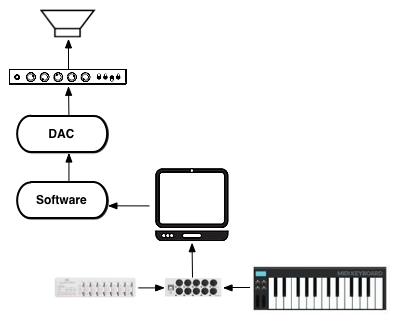
\includegraphics[scale=0.7]{../img/MIDI_1.png}
\end{center}

Initialize MIDI communication in SuperCollider.

\begin{lstlisting}[frame=single] 
MIDIClient.init;	
\end{lstlisting} 

Searching for physical and virtual midi devices connected to the computer. 

\begin{lstlisting}[frame=single] 
MIDIClient.sources;      // from
MIDIClient.destinations; // to
\end{lstlisting} 

\begin{itemize}
\tightlist
\item ports \(\rightarrow\) virtual and physical connectors.
\item channels
      \begin{itemize}
      \tightlist
      \item 16 for each port (as empty staff of a score).
      \item one channel can be mono or poli.
      \end{itemize}
\item voice \(\rightarrow\) instrument (timbre) that we assign to a channel.
\item message \(\rightarrow\) can be channel message or system message.
\end{itemize}

\href{img/MIDI_2.pdf}{More} on MIDI protocol. METTI LINK DI GITHUB

\subsection{Receive}\label{receive-midi}
Connect a MIDI device to the computer USB port (or a software to a virtual port).

\begin{enumerate}
\def\labelenumi{\arabic{enumi}.}
\tightlist
\item disconnect all MIDI message connections from/to SuperCollider (clean up).
\item connect all MIDI message connections from/to SuperCollider.
\begin{lstlisting}[frame=single] 
MIDIIn.disconnectAll; 
MIDIIn.connectAll;   
\end{lstlisting} 

\item check communication and the incoming message type.
\begin{lstlisting}[frame=single] 
MIDIFunc.trace(true);  // check message (Post window)
MIDIFunc.trace(false); // Stop checking
\end{lstlisting} 

\item choose the MIDI message type we want to receive.
\begin{lstlisting}[frame=single] 
MIDIdef.noteOn( \noteOn, {arg ...args; args.postln}); 
                        // velocity, note,      channel, uid
MIDIdef.noteOff(\noteOff,{arg ...args; args.postln}); 
                        // velocity, note,      channel, uid
MIDIdef.cc(     \control,{arg ...args; args.postln}); 
                        // value,   cc number,  channel, uid
\end{lstlisting} 
\end{enumerate}

\textit{MIDIdef} second argument ia a function that is evaluated each time a midi message is incoming.

Its argument is an array containing values from incoming message.

The values type depends on MIDI message type.

Main MIDI message types  \(\rightarrow\) \textit{.noteOn, .noteOff, .cc, .polytouch, .touch, .bend, .program, .sysex, .smpte, .sysrt}.

If you need more open \textit{MIDIdef} help file.

Kill one \textit{MIDIdef} or all. 
\begin{lstlisting}[frame=single] 
MIDIdef(\noteOn).free; // Cancella una specifica MIDIdef
MIDIdef.freeAll;       // Cancella tutte le MIDIdef
\end{lstlisting} 

If we want receive messages from a specific channel or control number.

\begin{lstlisting}[frame=single] 
MIDIdef.cc(\control_0,{arg val; val.postln});    // from all 
MIDIdef.cc(\control_1,{arg val; val.postln},1);  // only from cc 1 chan 0
MIDIdef.cc(\control_2,{arg val; val.postln},2);  // only from cc 2 chan 0
MIDIdef.cc(\control_3,{arg val; val.postln},3);  // only from cc 3 chan 0

MIDIdef.cc(\control_1,{arg val; val.postln},1,0);  // only from cc 1 chan 0
MIDIdef.cc(\control_2,{arg val; val.postln},1,1);  // only from cc 1 chan 1
MIDIdef.cc(\control_3,{arg val; val.postln},1,2);  // only from cc 1 chan 2
\end{lstlisting} 


\subsection{Send}\label{send-midi}

\begin{enumerate}
\def\labelenumi{\arabic{enumi}.}
\tightlist
\item search for available MIDI device destinations (Array of devices).
\item choose and set destination by index.
\item send MIDI messages.
\end{enumerate}

\begin{lstlisting}[frame=single] 
MIDIClient.destinations; 
c = MIDIOut.new(0);

//       channel,    pitch, velocity
c.noteOn(0,      rand(127), rand(127));
c.noteOff(0,     rand(127), rand(127));
c.allNotesOff(0);

//       channel, ccn,  val
c.control(0,        1,  rand(127));
\end{lstlisting} 

\subsection{Voice allocation}\label{voice-allocation}

There are three different Synth models designed for incoming midi message:

\begin{itemize}
\tightlist
\item monophonic.
\item poliphonic without sustain envelope (one message trigger + duration).
\item poliphonic with sustain envelope (two message switch - noteOn and noteOff).
\end{itemize}

They are usually triggered by keys or buttons but we can also control parameters with continuos signals from knobs, fader, etc.

\subsubsection{Monophonic synth}\label{monophonic-synth}

\begin{lstlisting}[frame=single] 
s.boot;
MIDIIn.disconnectAll;  
MIDIIn.connectAll;   
\end{lstlisting} 

The model

\begin{lstlisting}[frame=single, caption=MIDI monophonic instrument model] 
SynthDef(\midi, {arg freq=440, amp=0, gate=0, gain=0, pan=0; 
                 var sig, env;
                     sig = SinOsc.ar(freq);
                     env = Env.adsr;
                     env = EnvGen.kr(env,gate);
                     sig = sig * env * gain.lag(0.2); // lag 
                     sig = Pan2.ar(sig,pan);
                 Out.ar(0, sig)          
         }).add;

MIDIdef.cc(\masterOut, {arg val; // only first argument (cc value)
                        ~synth.set(\gain,val/127) // master out volume
           });
MIDIdef.noteOn(\noteOn,{arg vel,note;
                        ~synth.set(\freq,note.midicps, // MIDI to Hz
                                   \amp,vel/127,       // scaled amplitude
                                   \gate, 1);          // noteOn
           });
MIDIdef.noteOff(\noteOff,{~synth.set(\gate,0)});       // note off

~synth = Synth(\midi);

~port = MIDIOut.new(0);
~port.noteOn(0,  72, rand(127));
~port.control(0,  1,  64);
~port.control(0,  1,  rand(127));
~port.noteOff(0,     72, 0);
~synth.free; ~port.free; MIDIdef.freeAll;     
\end{lstlisting} 

\subsubsection{Poliphonic synth without sustain envelope}\label{poliphonic-synth-without-sustain-envelope}

Dynamic voice allocation.

Every time a MIDI message is received a new Synth instance is created.

After a defined time (duration) the instance is killed automatically (\textit{doneAction:2}).

Note off messages are not necessary (\textit{t\_gate}).

The model.

\begin{lstlisting}[frame=single, caption=MIDI poliphonic no-sustain instrument model] 
SynthDef(\midi_poli1, {arg freq=440, amp=0, dur=0.5, pan=0, t_gate=0;
                       var sig,env;
                           sig = Blip.ar(freq,40);
                           env = Env.perc(dur * 0.1,dur * 0.9);
                           env = EnvGen.kr(env,t_gate, doneAction:2);
                           sig = sig * env * amp;
                           sig = Pan2.ar(sig,pan);
                       Out.ar(0, sig)
          }).add;

MIDIdef.noteOn(\noteOn1,{arg vel, note;
                         Synth(\midi_poli1,[\freq,note.midicps,
                                            \amp,vel/127,
                                            \dur,1.5,
                                            \pan, rand2(1.0),
                                            \t_gate,1])
               })

~synth = Synth(\midi);

~port = MIDIOut.new(0);
~port.noteOn(0,  rrand(85,90), rand(127));
~port.free; MIDIdef.freeAll;      
\end{lstlisting} 

\subsubsection{Poliphonic synth with sustain envelope}\label{poliphonic-synth-with-sustain-envelope}

Static voice allocation.

We define an empty array with 128 items.

MIDI note \(\rightarrow\) array index (from 0 to 127).

Note On message \(\rightarrow\) put a Synth instance at index (pitch).

Note Off message \(\rightarrow\) send \textit{gate 0} to instance at index (pitch) and substitute the Synth with \textit{nil}.

\begin{lstlisting}[frame=single, caption=MIDI poliphonic w-sustain instrument model] 
SynthDef(\midi_poli2, {arg freq=789, amp=0, pan=0, gate=0;
                       var sig, env;
                           sig = SinOsc.ar(freq);
                           env = Env.adsr(0.01,0.3,0.5,1);
                           env = EnvGen.kr(env, gate, doneAction:2);
                           sig = sig * env * amp;
                           sig = Pan2.ar(sig, pan);
                       Out.ar(0, sig)
          }).add;

~note = Array.newClear(128); // Empty array with 128 items (all MIDI notes) 
                             // All elements are 'nil'

MIDIdef.noteOn(\noteOn1,{arg vel, pitch;
	                     ~note.put(pitch, 
                                   Synth(\midi_poli2,[\freq,pitch.midicps,
                                                      \amp,vel/127,
                                                      \gate,1]))
               });

MIDIdef.noteOff(\noteOff1,{arg vel, pitch;
	                       ~note.at(pitch).set(\gate,0);
	                       ~note.put(pitch, nil)
               });

~synth = Synth(\midi);

~port = MIDIOut.new(0);
~port.noteOn(0, rrand(80,90).postln, rand(40));
~port.noteOff(0, rrand(80,90), 0);   
~port.allNotesOff(0); ~port.free; ~note.free; MIDIdef.freeAll;
\end{lstlisting} 

\section{OSC}\label{osc}

Open Sound Control.

Born on 1997 CNMAT - Berkeley Univerity.

\begin{itemize}
\tightlist
\item communication procotol.
\item wireless.
\end{itemize}

We can connect electronic musical instruments, audio devices and computers without cables.

OSC message data types \(\rightarrow\) int32, float32 and strings.

\begin{center}
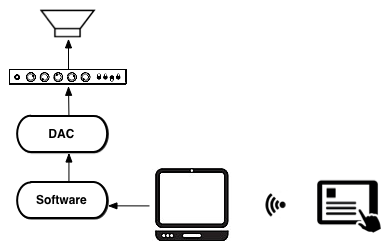
\includegraphics[scale=0.7]{../img/osc_1.png}
\end{center}

It is the protocol used in SuperCollider for communication between Interpreter and Server.

There are many smartphone and tablet app that support it.

You can use these devices as musical instrument controlling sound synthesi and processing in SuperCollider.

\href{https://hexler.net/touchosc}{TouchOsc} is a cheaper and powerful app.

\href{https://github.com/kylemcdonald/ofxFaceTracker/releases}{FaceOsc} can be useful to check communication between software in local machine.

There are not physical connections then we have to open one or more communication channels among devices and/or software setting an:

\begin{itemize}
\tightlist
\item IP address like "127.0.0.1" \(\rightarrow\) it uniquely identify a device.
\item OSC port \(\rightarrow\) an integer value that identify a monodirectional channel.
\end{itemize}

Each IP address can have many ports, usually for send and receive messages.

\subsection{Receive}\label{receive-osc}

Check communication and the incoming message type.

Server should be quit because we can monitor messages from Interpreter.

\begin{lstlisting}[frame=single] 
OSCFunc.trace(true);  // Check OSC messages
OSCFunc.trace(false); // Stop checking
\end{lstlisting} 

Messages are identified by a label starting with slash symbol.

Syntax is similar to the \textit{MIDIdef} class.

\begin{lstlisting}[frame=single] 
//            name,    function,            label       port
OSCdef.new(\criccio, {arg msg; msg.postln}, '/x',       recvPort:8001);
OSCdef.new(\ciaccio, {arg msg; msg.postln}, '/y',       recvPort:8001);
OSCdef.new(\ciuccio, {arg msg; msg.postln}, '/z',       recvPort:8001);
OSCdef.new(\cieccio, {arg msg; msg.postln}, '/1/fader1',recvPort:8001);

OSCdef(\criccio).free; 
OSCdef.freeAll;     
\end{lstlisting} 

\subsection{Send}\label{send-osc}

Set a device Net address.

Send messages to it.

\begin{lstlisting}[frame=single] 
c = NetAddr("127.0.0.0",  9000); // local address 

c.sendMsg("/fade1", rand(1.0));
c.sendMsg("/fade1", rand(1.0), rand(1.0), rand(1.0)); // send more than one value (array)  
\end{lstlisting} 

Check communication in local.

A send/receive model.

\begin{lstlisting}[frame=single] 
SynthDef(\osc, {arg freq=400,amp=0,pan=0,gate=0;
                var sig, env;
                    env = Linen.kr(gate,doneAction:2);
                    sig = SinOsc.ar(freq);
                    sig = sig * env * amp;
                    sig = Pan2.ar(sig, pan);    
                Out.ar(0,sig)
                }).add;

OSCdef.new(\gate, {arg msg;
                   a.set(\gate,msg[1]) },        
                   '/gate', recvPort:8000);

OSCdef.new(\osck, {arg msg;
                   msg.postln;
                   a.set(\freq,msg[1],\amp,msg[2],\pan,msg[3]) },        
                   '/osck', recvPort:8000);
                   
c = NetAddr("127.0.0.1",  8000); 
a = Synth(\osc,[\amp,0.5]);

c.sendMsg("/gate", 1);
c.sendMsg("/gate", 0); 
c.free;
\end{lstlisting} 

\section{HID}\label{hid}

Human Interface Device.

Devices designed for human-machine interaction $\rightarrow$ mouse, keyboard, joystick, graphic tablet, etc.

In SuperCollider two ways to receive values:

\begin{itemize}
\tightlist
\item Client side \(\rightarrow\) interaction in Interpreter (as MIDI and OSC).
\item Server side \(\rightarrow\) interaztion in Server (signals at control rate).
\end{itemize}

\subsection{Mouse}\label{mouse}

All the three control typologies: 

\begin{itemize}
\tightlist
\item trigger.
\item switch.
\item continuos.
\end{itemize}

\subsubsection{Client side}\label{mouse-client-side}

We must create a GUI window and interact with it.

Two reasons:

\begin{itemize}
\tightlist
\item avoid unwanted interactions.
\item delimit a space (range) for values.
\end{itemize}

Different methods for different actions.

\paragraph{.mouseDownAction} \(\rightarrow\) as for \textit{MIDIdef} and \textit{OSCdef} the function is evaluated each time a mouse button is clicked.

...args:

\begin{itemize}
\tightlist
\item 0 wiew \(\rightarrow\) the window clicked by mouse.
\item 1 x \(\rightarrow\) x position on widow in pixels (0 = leftmost).
\item 2 y \(\rightarrow\) y position on window in pixels (0 = higher). 
\item 3 modifiers \(\rightarrow\) if a modifier key is pressed.
\item 4 botton n \(\rightarrow\) botton number clicked (0=left, 1=right, 2=central).
\item 5 counter \(\rightarrow\) number of clicks (1=single click, 2 double click).
\end{itemize}

\begin{lstlisting}[frame=single, caption=mouseDownAction model] 
w = Window.new("mouse");
w.view.mouseDownAction_({arg ...args;
                                args.postln;    // all info
                                args[1].postln; // only x position
                       });
w.front;
w.alwaysOnTop_(true);
w.onClose_({w.free});
\end{lstlisting} 

Audio example.

\begin{itemize}
\tightlist
\item left click $\rightarrow$ trigger sine.
\item right click $\rightarrow$ trigger noise.
\end{itemize}

\begin{lstlisting}[frame=single] 
SynthDef.new(\sine, {arg freq=0, amp=0, t_gate=0;
                     var sig,env;
                         sig = SinOsc.ar(freq);
                         env = EnvGen.kr(Env.perc,t_gate,doneAction:2);
                     Out.ar(0,sig*env*amp);
             }).add;
SynthDef.new(\noise, {arg amp=0;
                      var sig;
                          sig = PinkNoise.ar;
                      Out.ar(0,sig*amp.lag(3));                  
             }).add;

w = Window.new("mouse");
w.view.mouseDownAction_({arg ...args;
                         if(args[4] == 0,    // if...
                         {Synth.new(\sine,
                                   [\freq, args[1].linlin(0,400,300,2000),
                                    \amp,1-args[2].linlin(0,400,0,1.0),
                                    \t_gate, 1])}, 
		                 {a.set(\amp, 1-args[2].linlin(0,400,0,1.0))})                                  
                         });
w.front;
w.alwaysOnTop_(true);
w.onClose_({w.free;s.freeAll});

a = Synth.new(\noise);
\end{lstlisting} 

\paragraph{.mouseUpAction} \(\rightarrow\) as previous but function is evaluated when button is released.

\begin{lstlisting}[frame=single, caption=mouseUpAction model] 
w = Window.new("mouse");
w.view.mouseUpAction_({arg ...args;
                              args.postln;    // all info
                              args[1].postln; // only x position
                       });
w.front;
w.alwaysOnTop_(true);
w.onClose_({w.free});
\end{lstlisting} 

Audio example.

\begin{itemize}
\tightlist
\item left click $\rightarrow$ trigger sine (trigger).
\item right click $\rightarrow$ fade in noise (switch).
\item right release$\rightarrow$ fade out noise.
\end{itemize}

\begin{lstlisting}[frame=single] 
SynthDef.new(\sine, {arg freq=0, amp=0, t_gate=0;
                     var sig,env;
                         sig = SinOsc.ar(freq);
                         env = EnvGen.kr(Env.perc,t_gate,doneAction:2);
                     Out.ar(0,sig*env*amp);
             }).add;
SynthDef.new(\noise, {arg amp=0;
                      var sig;
                          sig = PinkNoise.ar;
                      Out.ar(0,sig*amp.lag(0.2)); // fade di 0.2 secondi
             }).add;

w = Window.new("mouse");
w.view.mouseDownAction_({arg ...args;
                         if(args[4] == 0,
                         {Synth.new(\sine,
                                   [\freq, args[1].linlin(0,400,300,2000),
                                    \amp,1-args[2].linlin(0,400,0,1.0),
                                    \t_gate, 1])}, 
		                 {a.set(\amp, args[2].linlin(0,400,0,1.0))}) // note On                      
                         });
w.view.mouseUpAction_({arg ...args;
                              args.postln;
                              a.set(\amp, 0) // note Off                             
                       });
w.front;
w.alwaysOnTop_(true);
w.onClose_({w.free;s.freeAll});

a = Synth.new(\noise)
\end{lstlisting} 

\paragraph{.mouseMoveAction} \(\rightarrow\) as previous but if we click and draw values change dynamically in a continuos way.

Top-left corner \(\rightarrow\) (0, 0)

Out of window positions \(\rightarrow\) negative or positive values.

\begin{lstlisting}[frame=single, caption=mouseMoveAction model] 
w = Window.new("mouse");
w.view.mouseMoveAction_({arg ...args;
                                args.postln;    // all info
                                args[1].postln; // only x position
                       });
w.front;
w.alwaysOnTop_(true);
w.onClose_({w.free});
\end{lstlisting} 

Audio example.

\begin{itemize}
\tightlist
\item click and release \(\rightarrow\) switch (noteOn and noteOff).
\item draw \(\rightarrow\) continuos values.
\end{itemize}

\begin{lstlisting}[frame=single] 
SynthDef.new(\spectra, {arg freq=0, amp=0, harm=1, gate=0;
                        var sig,env;
                            sig = Blip.ar(freq,harm);
                            env = EnvGen.kr(Env.asr(0.3,1,5),gate,doneAction:2);
                        Out.ar(0,sig*env*amp);
             }).add;

w = Window.new("mouse");
w.view.mouseDownAction_({arg ...args;                  // note On 
                         a = Synth.new(\spectra, 
                                      [\freq, args[1].linlin(0,400,300,2000),
                                       \gate, 1]);
                         });
w.view.mouseMoveAction_({arg ...args;                 // continuos signal
	                     a.set(\amp,1-args[2].linlin(0,400,0,1.0),
		                       \harm, args[1].linlin(0,400,1,20))
                         });
w.view.mouseUpAction_({arg ...args;
                       a.set(\gate,0)                  // note Off
                      });
w.front;
w.alwaysOnTop_(true);
w.onClose_({w.free;s.freeAll});
\end{lstlisting} 

\paragraph{.mouseOverAction} \(\rightarrow\) as previous but without click (passing mouse on the window).

Top-left corner \(\rightarrow\) (0, 0)

Out of window positions \(\rightarrow\) negative or positive values.

\begin{lstlisting}[frame=single, caption=mouseOverAction model] 
w = Window.new("mouse");
w.view.mouseOverAction_({arg ...args;
                                args.postln;    // all info
                                args[1].postln; // only x position
                       });
w.front;
w.alwaysOnTop_(true);
w.onClose_({w.free});
\end{lstlisting} 

Audio example.

\begin{lstlisting}[frame=single] 
b = Buffer.read(s, "/absolute/path/to/file.wav");
SynthDef.new(\scratch, {arg pos=0, amp=0, buf=0, smooth=0.2;
                        var sig, punt;
                            punt = BufFrames.ir(buf)*K2A.ar(pos).varlag(smooth);
                            sig  = BufRd.ar(1,b,punt);
                        Out.ar(0,sig*amp.lag(0.2))
              }).add;

w = Window.new("mouse").acceptsMouseOver_(true); 
w.view.mouseOverAction_({arg ...args;
                         a.set(\pos, args[1].linlin(0,400,0,1),    // x pos
                               \amp,1-args[2].linlin(0,400,0,1.0)) // y pos
                        });
w.front;
w.alwaysOnTop_(true);
w.onClose_({w.free;a.free;b.free});

a = Synth.new(\scratch, [\buf,b]);	
\end{lstlisting} 

\subsubsection{Server side}\label{mouse-server-side}

It's not necessary a GUI window.

Screen boundaries.

Three UGens:

\begin{itemize}
\tightlist
\item \textit{MouseX.kr} \(\rightarrow\) min, max, curve, lag time.
\item \textit{MouseY.kr} \(\rightarrow\) min, max, curve, lag time.
\item \textit{MouseButton} \(\rightarrow\) min, max, lag time.
\end{itemize}

\begin{lstlisting}[frame=single, caption=mouse controls Server model] 
{[MouseX.kr(0,1,0,0.2), MouseX.kr(0.0001,1,1,0.2)]}.scope; // lin vs exp
{[MouseY.kr(0,1,0,5),   MouseY.kr(0.0001,1,1,5)]}.scope;   // 5 sec lag time	
{[MouseButton.kr(0,1,0.1),   MouseButton.kr(0,1,)]}.scope; // 3 sec lag time
\end{lstlisting} 

Audio example.

\begin{lstlisting}[frame=single] 
b = Buffer.read(s, "/absolute/path/to/file.wav");
SynthDef.new(\scratch, {arg gate=1, buf;
                        var sig, speed, env;
                            env   = Env.new([0,1,0], 
                                            [0.1, 0.1], 
                                            \sin, 1).kr(20,gate);
                            speed = MouseX.kr(-10, 10);
                            speed = speed - DelayN.kr(speed, 0.1, 0.1);
                            speed = MouseButton.kr(1, 0, 0.3) + speed ;
                            sig   = PlayBuf.ar(1, buf, 
                                               speed * BufRateScale.kr(buf), 
                                               loop: 1);
                        Out.ar(0, sig * env );
              }).add;

a = Synth.new(\scratch, [\buf, b]);	
a.set(\gate, 0); a.free; b.free;
\end{lstlisting} 

\subsection{Keyboard}\label{keyboard}

Only two control typologies: 

\begin{itemize}
\tightlist
\item trigger \(\rightarrow\) press and release the key quickly. .
\item switch \(\rightarrow\) press and release.
\end{itemize}

\subsubsection{Client side}\label{key-client-side}

We must create a GUI window and interact with it.

The reason is avoid unwanted code writing.

Different methods for different actions.

\paragraph{.keyDownAction} \(\rightarrow\) as for \textit{MIDIdef} and \textit{OSCdef} the function is evaluated each time a key is clicked.

...args:

\begin{itemize}
\tightlist
\item 0 wiew \(\rightarrow\) the window clicked by mouse.
\item 1 char \(\rightarrow\) pressed character.
\item 2 modifiers \(\rightarrow\)  if a modifier key is pressed.
\item 3 unicode \(\rightarrow\) unicode value (\href{https://ss64.com/ascii.html}{ASCII}).
\item 4 keycode \(\rightarrow\) \href{https://www.toptal.com/developers/keycode}{keycode} value (JavaScript).
\item 5 key \(\rightarrow\) deprecated.
\end{itemize}

\begin{lstlisting}[frame=single, caption=keyDownAction model] 
w = Window.new("key");
w.view.keyDownAction_({arg ...args;
                              args.postln;
                              args[1].postln
                       });
w.front;
w.alwaysOnTop_(true);
w.onClose_({w.free})
\end{lstlisting} 

Audio example (trigger).

\begin{lstlisting}[frame=single] 
SynthDef.new(\if_1, {arg t_gate=0;
                     var sig, env;
                         sig = Saw.ar([600,602]);
                         env = EnvGen.ar(Env.perc,t_gate,doneAction:2);
                     Out.ar(0,sig*env);
         }).add;

w = Window.new("key");
w.view.keyDownAction_({arg ...args;
                           if(args[1]==$q, {Synth(\if_1, [\t_gate,1])}) 
                       });
w.front;
w.alwaysOnTop_(true);
w.onClose_({w.free});
\end{lstlisting} 

\paragraph{.keyUpAction} \(\rightarrow\) as previous but function is evaluated when key is released.

\begin{lstlisting}[frame=single, caption=keyUpAction model] 
w = Window.new("key");
w.view.keyUpAction_({arg ...args;
                            args.postln;
                            args[1].postln
                       });
w.front;
w.alwaysOnTop_(true);
w.onClose_({w.free})
\end{lstlisting} 

If we hold down a key we obtain redundant data.

\begin{lstlisting}[frame=single] 
SynthDef.new(\if_1, {arg t_gate=0;
                     var sig, env;
                         sig = Saw.ar;
                         env = EnvGen.ar(Env.perc,t_gate);
                     Out.ar(0,sig*env);
             }).add;

w = Window.new("key");
w.view.keyDownAction_({arg ...args;
	                   if(args[1]==$q, {a.set(\t_gate,1)}); // 'q' = Note On
                       });
w.view.keyUpAction_({arg ...args;
	                 if(args[1]==$q,{a.set(\t_gate,0)});    // Note Off
                     });
w.front;
w.alwaysOnTop_(true);
w.onClose_({w.free;a.free});
a = Synth.new(\if_1);
\end{lstlisting} 

To avoid \(\rightarrow\) filter incoming data.

\begin{lstlisting}[frame=single] 
var ora, prec = 0;                           // variable init
w = Window.new("key");
w.view.keyDownAction_({arg ...args;
                       ora = args[3];
                       if((ora != prec), // if different from previuos
                       {"noteOn".postln; // play and
                        prec = ora });   // assign 'prec' to last received value
                       });                   
					   
w.view.keyUpAction_({
                     prec = 0;         // reset Array 
                     "noteOff".postln; // Action
                     });            
w.front;
w.alwaysOnTop_(true);
w.onClose_({w.free})
\end{lstlisting} 

Audio example (switch).

\begin{lstlisting}[frame=single] 
SynthDef.new(\if_1, {arg gate=0;
                     var sig, env;
                         sig = Saw.ar;
                         env = EnvGen.ar(Env.adsr,gate,doneAction:2);
                     Out.ar(0,sig*env);
             }).add;

~ora;
~prec = 0;
w     = Window.new("key");
w.view.keyDownAction_({arg ...args;   // 'q' = Note On
                           ~ora = args[1];
                           if(        // if = 'q' AND != from previous
                           (~ora == $q).and(~ora != ~prec),
                           {a = Synth.new(\if_1, [\gate,1]);
                           ~prec = ~ora})
                       });
w.view.keyUpAction_({                            // Note Off
                     if(~ora==$q, {a.set(\gate,0);
                                   ~prec = 0});  // Reset
                     });
w.front;
w.alwaysOnTop_(true);
w.onClose_({w.free;a.free});
\end{lstlisting} 

\subsubsection{Server side}\label{key-server-side}

It's not necessary a GUI window (but suggested).

One UGen:

\begin{itemize}
\tightlist
\item \textit{KeyStart.kr} \(\rightarrow\) min, max, lag time.
\end{itemize}

We must know keycode in advance.

\begin{lstlisting}[frame=single, caption=key control Server model] 
w = Window.new;
w.front;
SynthDef.new(\key, {var amp,sig;
                        amp = KeyState.kr(38,0,1.0);   // 'j' key
                        sig = SinOsc.ar * amp;
                    Out.ar(0,sig)
            }).add;

Synth.new(\key); 
\end{lstlisting} 

\section{Live playback and synthesis}\label{Live-playback-and-synthesis}

If we want playback sound files or trigger synthesis sounds or sequences in a perforance we can:

\begin{itemize}
\tightlist
\item one-shot \(\rightarrow\) play it from beginning to end (old school).
\item map key (HID, MIDI or OSC) \(\rightarrow\) event (soundfile or other).
     \begin{itemize}
     \tightlist
     \item key \(\rightarrow\) trig soundfile or Synth.
     \item key \(\rightarrow\) set playback rate (sampler-like transposition) or other parameters.
     \item key \(\rightarrow\) set start position (and duration) in a soundfile.
     \end{itemize}
\item play it in a sequential way (cues + counter).
     \begin{itemize}
     \tightlist
     \item cue \(\rightarrow\) trig soundfile or Synth.
     \item cue \(\rightarrow\) set start position (and duration) in a soundfile or other parameters.
     \end{itemize}
\end{itemize}

\subsection{One shot}\label{one-shot}

The old tape playback.

If we want to sync it with live player parts we need to write it on the score in two ways:

\begin{enumerate}
\def\labelenumi{\arabic{enumi}.}
\tightlist
\item a seconds grid (chronometric way).
\begin{center}
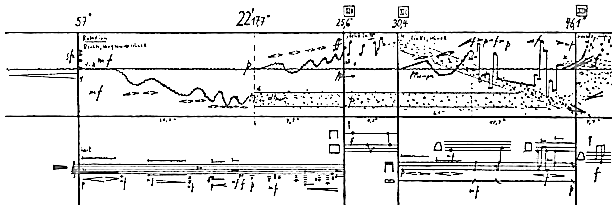
\includegraphics[scale=0.9]{../img/kont.png}
\end{center}

\item a graphic representation staff (waveform or sonogram).
\begin{center}
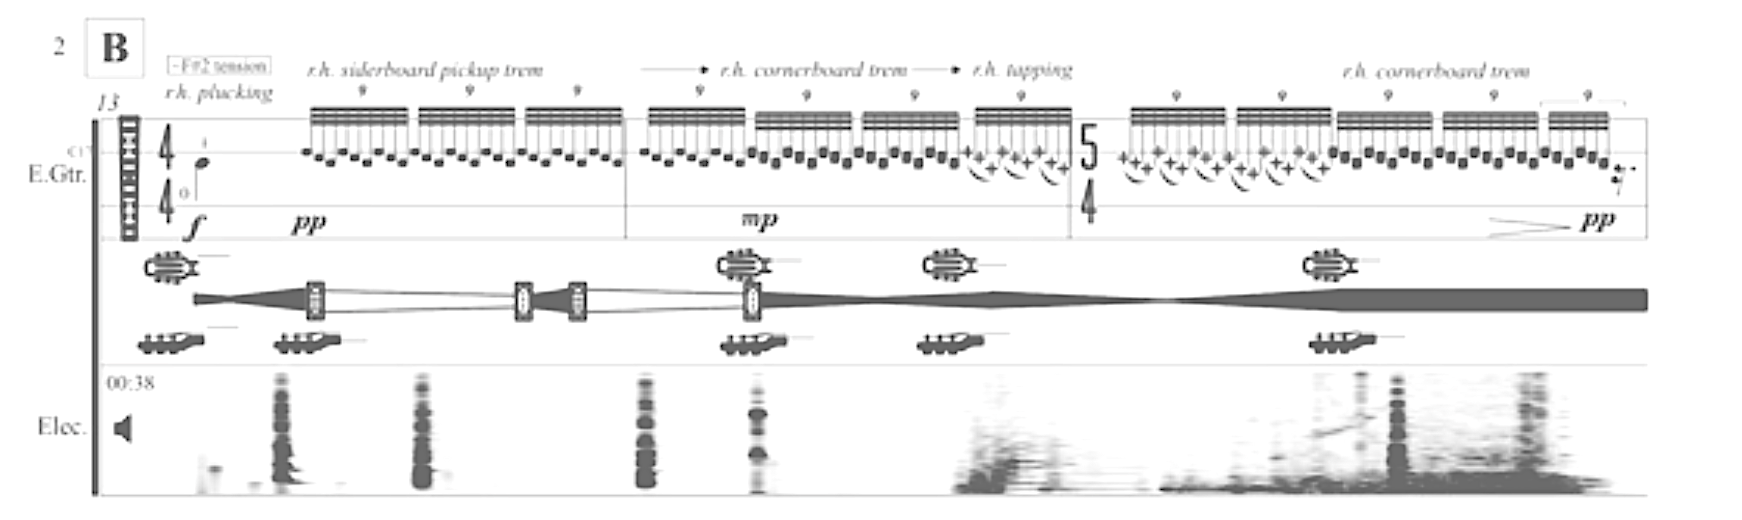
\includegraphics[scale=0.9]{../img/kokoras.png}
\end{center}

We can create a click-track for live performers.

Both are rigid and difficult systems in syncro for live player.

Good for metrical grid rhythms (pop and rock music).

Bad for rapsodic music.

Complicated for rehearsals.

Only start and stop actions.

We can control it by a triggered switch on asingle key.

\begin{lstlisting}[frame=single, caption=playback one-shot model] 
b = Buffer.read(s, "/absolute/path/to/voce.wav");
SynthDef.new(\simple_player, {arg buf=0, amp=0, pan=0, gate=0;
                              var env, sig;
                                  env = Linen.kr(gate, doneAction:2);
                                  sig = PlayBuf.ar(1, buf, 
                                                   BufRateScale.kr(buf), 
                                                   doneAction:2);
                                  sig = sig * env * amp.lag(0.2);
                                  sig = Pan2.ar(sig, pan); 
	                         Out.ar(0, sig);
              }).add;

w = Window.new("key");
~switch = [1,0]; // Flip flop
~synth;
w.view.keyDownAction_({arg ...args;
                       if(args[3]==32){
                                       if(~switch.first==1)
                                       {~synth = Synth.new(\simple_player,
                                                           [\buf,b,
                                                            \amp,1,
                                                            \gate,1])}
                                       {~synth.set(\gate,0)};
                                       ~switch = ~switch.reverse;
                                       }
                       });
w.front;
w.alwaysOnTop_(true);
w.onClose_({w.free;a.free});
\end{lstlisting} 

\end{enumerate}
\subsection{Mapping}\label{mapping}

We can map an event (soundfile or other) to a key as a piano keyboard or bandoneon button.

\begin{center}
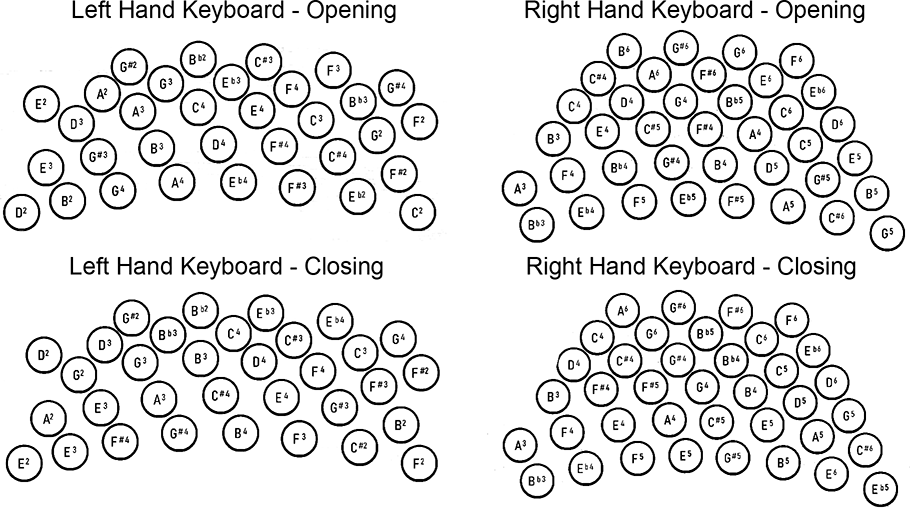
\includegraphics[scale=0.9]{../img/mapping.png}
\end{center}

\subsubsection{Key \(\rightarrow\) soundfile }\label{key-soundfile}

Load all soundfiles in a folder in one array of Buffers.

Soundfile durations should be short (no stop command).

\begin{lstlisting}[frame=single, caption=playback key-map-soundfile model] 
~paths = ("/absolute/path/to/folder" ++ "/*.wav").pathMatch;
~bufs  = ~paths.collect{arg i; Buffer.read(s, i)};

SynthDef.new(\map_player, {arg buf=0, amp=0, pan=0;
                           var sig;
                               sig = PlayBuf.ar(1, buf, 
                                                BufRateScale.kr(buf), 
                                                doneAction:2);
                               sig = sig * amp;
                               sig = Pan2.ar(sig, pan); 
                           Out.ar(0, sig);
              }).add;

w = Window.new("key");
w.view.keyDownAction_({arg ...args;
	                    switch(args[1],
	                    $q, {Synth.new(\map_player,[\amp,0.5, \buf,~bufs[0]])},
	                    $w, {Synth.new(\map_player,[\amp,0.5, \buf,~bufs[1]])},
	                    $e, {Synth.new(\map_player,[\amp,0.5, \buf,~bufs[2]])},
	                    $r, {Synth.new(\map_player,[\amp,0.5, \buf,~bufs[3]])},
	                    $t, {Synth.new(\map_player,[\amp,0.5, \buf,~bufs[4]])} );
                       });
w.front;
w.alwaysOnTop_(true);
w.onClose_({w.free;a.free});
\end{lstlisting} 

\subsubsection{Key \(\rightarrow\) playback rate (transposition) }\label{key-rate}

One soundfile.

Transposition in semitones.

\begin{lstlisting}[frame=single, caption=playback key-playback-rate model] 
b = Buffer.read(s, "/absolute/path/to/voce.wav");
SynthDef.new(\smp_player, {arg buf=0, amp=0, trsp=0, pan=0;
                           var sig;
                               sig = PlayBuf.ar(1, buf,
                                                trsp.midiratio*BufRateScale.kr(buf), 
                                                doneAction:2);
                               sig = sig * amp;
                               sig = Pan2.ar(sig, pan);
                           Out.ar(0, sig);
              }).add;

w = Window.new("key");
w.view.keyDownAction_({arg ...args;
                      switch(args[1],
                      $q, {Synth.new(\smp_player,[\amp,0.5, \buf,b,\trsp,-4])},
                      $w, {Synth.new(\smp_player,[\amp,0.5, \buf,b,\trsp, 0])},
                      $e, {Synth.new(\smp_player,[\amp,0.5, \buf,b,\trsp, 2])},
                      $r, {Synth.new(\smp_player,[\amp,0.5, \buf,b,\trsp, 3])},
                      $t, {Synth.new(\smp_player,[\amp,0.5, \buf,b,\trsp, 5])},
                      $y, {Synth.new(\smp_player,[\amp,0.5, \buf,b,\trsp, 7])},                            
                      );
                      });
w.front;
w.alwaysOnTop_(true);
w.onClose_({w.free;a.free});
\end{lstlisting} 

\subsubsection{Key \(\rightarrow\) start position }\label{key-start-position}

One soundfile.

Positions and durations in seconds.

\begin{lstlisting}[frame=single, caption=playback key-start-position model] 
b = Buffer.read(s, "/absolute/path/to/voce.wav");
SynthDef.new(\pos_player, {arg buf=0, amp=0, pos=0, dur=0.5, pan=0;
                           var env, sig;
                               env = Env.linen(0.01,dur-0.02,0.01);
                               env = EnvGen.kr(env,doneAction:2);
                               sig = PlayBuf.ar(1, buf, 
                                                BufRateScale.kr(buf),
                                       startPos:pos*BufSampleRate.kr(buf));
                               sig = sig * env * amp;
                               sig = Pan2.ar(sig, pan);
                           Out.ar(0, sig);
              }).add;

w = Window.new("key");
w.view.keyDownAction_({arg ...args;
                       switch(args[1],
                       $q, {Synth.new(\pos_player,[\amp,0.5, \buf,b,
                                                   \pos,0,   \dur,1])},
                       $w, {Synth.new(\pos_player,[\amp,0.5, \buf,b,
                                                   \pos,1,   \dur,0.5])},
                       $e, {Synth.new(\pos_player,[\amp,0.5, \buf,b,
                                                   \pos,2,   \dur,0.2])},
                       $r, {Synth.new(\pos_player,[\amp,0.5, \buf,b,
                                                   \pos,3,   \dur,0.3])},
                       $t, {Synth.new(\pos_player,[\amp,0.5, \buf,b,
                                                   \pos,4,   \dur,0.4])}     
                       );
                       });
w.front;
w.alwaysOnTop_(true);
w.onClose_({w.free;a.free});
\end{lstlisting} 

\subsection{Cues}\label{cues}

We can set events in a sequential order and recall it during performance by number.

\begin{center}
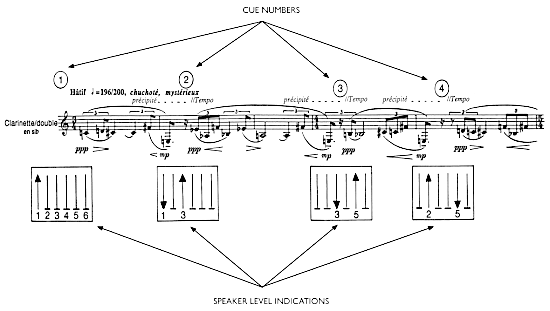
\includegraphics[scale=0.9]{../img/dialogue.png}
\end{center}

We need to program a counter.

A usual strategy is program also a cross playback with two alternate players.

\begin{center}
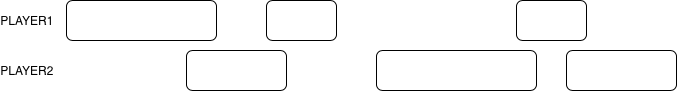
\includegraphics[scale=0.9]{../img/cross.png}
\end{center}

This need a crossfade at trigger point.

More dynamic than one-shot playback and better for rehearsals.

Cue durations should be between 1 and 10-15 seconds.

\begin{lstlisting}[frame=single, caption=playback cues model] 
~paths = ("/absolute/path/to/folder" ++ "/*.wav").pathMatch;
~bufs  = ~paths.collect{arg i; Buffer.read(s, i)};

SynthDef(\cross, {arg buf=0, amp=0, fade=0.1, pan=0, gate=0;
                  var sig,dur,fad,env;
                      sig = PlayBuf.ar(2, buf);
                      dur = BufDur.kr(buf);
                      fad = Linen.kr(gate,fade,amp.lag(0.2),fade,doneAction:2);     
                      env = EnvGen.kr(Env.linen(0.2,dur-0.4,0.2),
                                      gate,doneAction:2);
                      sig = sig * env * fad;
                      sig = Pan2.ar(sig,pan); 
                  Out.ar(0,sig)
         }).add;

~cue = 0; // Init counter

w = Window.new("Num", Rect.new(0,0,300,300));
h = NumberBox.new(w, Rect(5,5,290,290))
             .align_(\center)
             .font_(Font("Helvetica", 200););

w.front;
w.alwaysOnTop_(true);
w.onClose_({w.free;h.free; ~cue.free});

w.view.keyDownAction_({arg ...args;
                       switch(args[3],
                       32, {         // space bar --> increment
                            h.value = ~cue;                         // visualization
                            if(s.numSynths > 0, {a.set(\gate,0)});  // Fade out               
                            a = Synth(\cross, [\fade, 2, 
                                               \amp, 1, 
                                               \buf, ~bufs[~cue],
                                               \gate,1]);
                            ~cue  = ~cue + 1 % ~bufs.size;          // modulo increment
                            },
                       105, {~cue = 0;                             // 'i' --> reset to 0
                             h.value = 0;
                             if(s.numSynths > 0, {a.set(\gate,0)}); })
                       });
					   
h.action_({arg val; ~cue = val.value}); // we can set cue on GUI
\end{lstlisting} 

All the examples are with soundfiles players but we can subtitute it with any type of live synthesis generator.

All the examples are triggered by computer key but we can use any kind of controller (MIDI, OSC, mouse, etc.).

\section{Composition sketches proposal}\label{composition-sketches-proposal}

\begin{itemize}
\tightlist
\item design and build a live set with available tools (MIDI, OSC, HID; etc.).

      Keep in mind:
      \begin{itemize}
      \tightlist
      \item sound palette  we want to have (sound synthesis and processing techniques).
      \item which and how many parameters we want to control.
      \item how do we want to control them (knob, fader, botton, accelerometer, gyroscope, etc.).
      \item type of interaction (physical and musical gestures) we want to use.
      \end{itemize}
\item define a performance that can be:
      \begin{itemize}
      \tightlist
      \item written in a gestural score (we write in a time grid the gestures to be made live on the devices).
      \item improvised by interpreting a graphic score.
      \item totally improvised in search of the possibilities offered by the performance environment according to the principe of free will.
      \end{itemize}

\item performance can be in solo or in laptop ensemble. 

      If you play it in ensemble ypu should think about:
      \begin{itemize}
      \tightlist
      \item differentiate or sonically and musically unify the individual sets.
      \item what kind of strategies to adopt for synchronisation.
      \item have a conductor or not.
      \end{itemize}
\end{itemize}
